\clearpage
\Question[2]{Pointer Illustration}\TAGS{aliasing, memory-model, pointer}

Clearly and carefully illustrate the contents of memory after the
following code runs. We've drawn the contents of \lstinline'w', a pointer
that points into allocated memory where the number 0 is stored.

\smallskip
\begin{lstlisting}
int* w = alloc(int);
int i = 42;
int* p = alloc(int);
int* q = p;
int* r = alloc(int);
int** x = alloc(int*);
int** y = x;
int** z = alloc(int*);
*r = i + 7;
*x = q;
**y = *r - i;
p = NULL;
*z = r;
i = *q + **x + *w;
\end{lstlisting}

\bigskip

\begin{framed}
\ifprintanswers{\color{\answerColor}
\begin{lstlisting}[aboveskip=0pt, belowskip=0pt, lineskip=-0.2ex]
    ___       ___
   |   |     |   |
 w | *------>| 0 |
   |___|     |___|
   |   |
 i | 14|
   |___|
   |   |
 p | *---||   ___
   |___|     |   |
   |   |   />| 7 |<--\
 q | *----/  |___|    |
   |___|      ___     |
   |   |  /->|   |    |
 r | *---/   | 49|<--------\
   |___|     |___|    |     |
   |   |              |     |
 x | *---\    ___     |     |
   |___|  \->|   |    |     |
   |   |  /->| *-----/      |
 y | *---/   |___|          |
   |___|      ___           |
   |   |     |   |          |
 z | *------>| *-----------/
   |___|     |___|
\end{lstlisting}
}\else
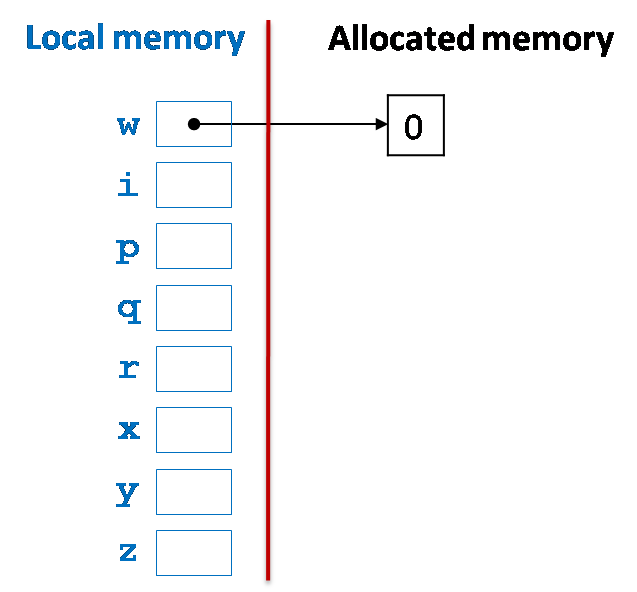
\includegraphics[width=0.82\textwidth]{\img/template.png}
\fi
\end{framed}

\RUBRIC
TAGS: aliasing, memory-model, pointer

Gradescope rubric:
+1pt i, p, *q, and *r are 14, NULL, 7, and 49, respectively
+1pt EITHER r == *z, x == y, *y == q
+0.5pt   OR no more than 2 incorrect arrows

Commentary:
    ___       ___
   |   |     |   |
 w | *------>| 0 |
   |___|     |___|
   |   |
 i | 14|
   |___|
   |   |
 p | *---||   ___
   |___|     |   |
   |   |   />| 7 |<--\
 q | *----/  |___|    |
   |___|      ___     |
   |   |  /->|   |    |
 r | *---/   | 49|<--------\
   |___|     |___|    |     |
   |   |              |     |
 x | *---\    ___     |     |
   |___|  \->|   |    |     |
   |   |  /->| *-----/      |
 y | *---/   |___|          |
   |___|      ___           |
   |   |     |   |          |
 z | *------>| *-----------/
   |___|     |___|

1 point
  . i, *p, and *r return the correct answers, q is NULL
  . All or nothing (this was easy for them to test)
1 point - Structure is correct: p == q, y == z, *x == r, *y == p
  . Half of this point if no more than two structure arrows are wrong
ENDRUBRIC
